\documentclass[margin=2pt]{standalone}
\usepackage[table]{xcolor}
\usepackage[utf8]{inputenc}
\usepackage[T1]{fontenc}

\usepackage{tikz}
\usepackage{helvet}
\usepackage{amsmath}

\renewcommand\familydefault\sfdefault

% Use \phantom to hide text for exams
\renewcommand{\phantom}{}

\newcommand{\lCPU}{CPU}
\newcommand{\lLimit}{LA > Limit?}
\newcommand{\lLimitError}{Chyba narušení\\ochrany}
\newcommand{\lMemory}{Paměť} % \phantom{}
\newcommand{\lFAP}{FAP}
\newcommand{\lAddressLogical}{\phantom{Logická}\\{adresa}}
\newcommand{\lAddressPhysical}{\phantom{Fyzická}\\{adresa}}
\newcommand{\lRegLimit}{\phantom{Limitní}\\(mezní)\\registr}
\newcommand{\lRegBase}{Realokační\\(\phantom{bázový})\\registr}

\usetikzlibrary{intersections, shapes.arrows, spath3, shapes.geometric, fit, backgrounds, calc, tikzmark}

\definecolor{themeBlue}{RGB}{1, 103, 143}
\definecolor{themeOrange}{RGB}{221, 109, 16}
\definecolor{themeTeal}{RGB}{18, 54, 69}
\definecolor{themeGrey}{RGB}{120, 121, 124}

\begin{document}
    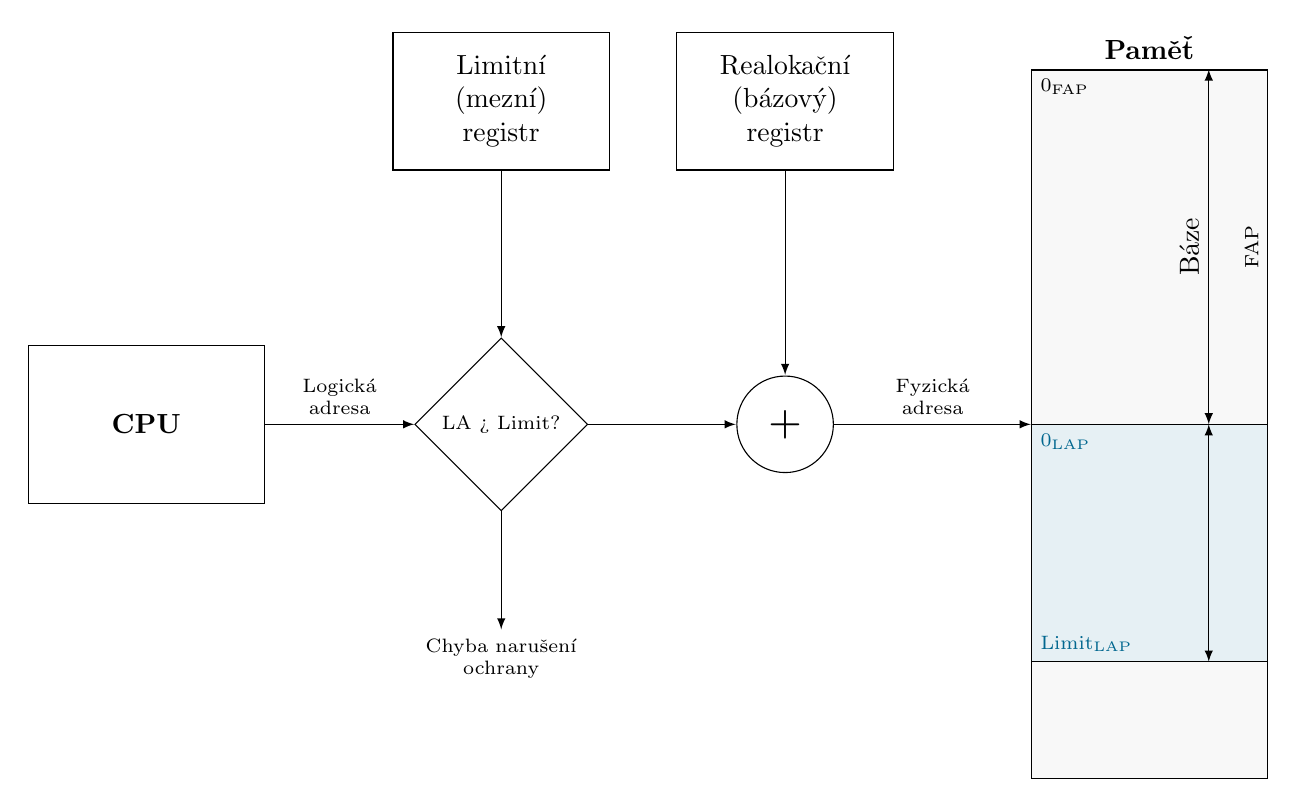
\begin{tikzpicture} [
        %font=\small,
        cpu/.style={draw, minimum width=3cm, minimum height=2cm, align=center, font=\bfseries},
        reg/.style={draw, minimum width=2.75cm, minimum height=1.75cm, align=center},
        mem/.style={draw, minimum width=3cm, minimum height=9cm, fill=themeGrey!5},
        mem check/.style={draw, diamond, align=center, font=\scriptsize},
        mem block/.style={draw, anchor=north, minimum width=3cm, minimum height=3cm, fill=themeBlue!10},
        sum address/.style={draw, circle, align=center, font=\scriptsize, scale=2},
        limit error/.style={below, minimum width=2cm, align=center, font=\scriptsize},
        label address/.style={midway, above, align=center, font=\scriptsize},
        label LAP/.style={right, font=\scriptsize, text=themeBlue},
        label mem/.style={above, font=\bfseries}
    ]

    \path node[cpu] (cpu) {$ \text{\lCPU} $};
    \path (cpu.east) ++(3cm,0) node[mem check] (is limit?) { \lLimit };
    \path (is limit?.north) ++(0, 3cm) node[reg] (reg lim) { \lRegLimit };
    \path (is limit?.east) ++(2.5cm,0) node[sum address] (add sum) {$ + $};
    \path (add sum.north|-reg lim.north) node[reg, anchor=north] (reg base) { \lRegBase };
    \path (add sum.east) ++(4cm, 0) node[mem] (mem) {};
    \path (mem|-add sum) node[mem block] (mem block) {};


    \path (mem.north) node[label mem] {$ \text{\lMemory} $};
    \path ($ (mem.north east)!.5!(mem block.north east) $) node[above, rotate=90, font=\scriptsize] {$ \text{\lFAP} $};
    \path (mem.north west) node[below, right, anchor=north west, font=\scriptsize] {$ \text{0}_{\text{FAP}} $};

    \path (mem block.north west) node[label LAP, below, anchor=north west] {$ \text{0}_{\text{LAP}}
    $};
    \path (mem block.south west) node[label LAP, above, anchor=south west] {$ \text{Limit}_{\text{LAP}} $};
    
    \draw[latex-latex] ($ (mem.north west)!.75!(mem.north east) $) -- node[midway, above, rotate=90] {Báze} ($ (mem block.north west)!.75!(mem block.north east) $);
    \draw[latex-latex] ($ (mem block.north west)!.75!(mem block.north east) $) -- ($ (mem block.south west)!.75!(mem block.south east) $);

    \draw[-latex] (cpu.east) -- node [label address] {\lAddressLogical} (is limit?.west);
    \draw[-latex] (reg lim.south) -- (is limit?.north);
    \draw[-latex] (is limit?.east) -- (add sum.west);
    \draw[-latex] (reg base.south) -- (add sum.north);
    \draw[-latex] (add sum.east) -- node [label address] {\lAddressPhysical} (mem.west);
    \draw[-latex] (is limit?.south) -- ++(0, -1.5cm) node[limit error] {\lLimitError};

    \end{tikzpicture}
\end{document}